%\section*{Đề thi thử THPTQG Sở GD\& ĐT 25--26, Lần 1}
\caulc
\Opensolutionfile{ans}[ans/ans-62-26-2-HaNoi-KimLien-L3-LC]

\begin{ex}%[1D6H2-1]
	Với $a$ là số thực dương tùy ý và $a \ne 1$, giá trị của biểu thức $P = \log_{\sqrt{a}}(a^3 \cdot \sqrt{a})$ bằng
	\choice
	{\True $7$}
	{$\dfrac{4}{3}$}
	{$\dfrac{2}{7}$}
	{$\dfrac{8}{3}$}
	\loigiai{
		Ta có: $a^3 \cdot \sqrt{a} = a^3 \cdot a^{\frac{1}{2}} = a^{\frac{7}{2}}$ và $\sqrt{a} = a^{\frac{1}{2}}$. \\
		Do đó: $P = \log_{a^{\frac{1}{2}}}\left(a^{\frac{7}{2}}\right) = \dfrac{\frac{7}{2}}{\frac{1}{2}} \log_a a = 7$.
	}
\end{ex}

\begin{ex}%[2D1N3-1]
	\immini{Cho hàm số $y=f(x)$ liên tục trên đoạn $[-1;5]$ và có đồ thị như hình vẽ. Tổng giá trị lớn nhất và giá trị nhỏ nhất của hàm số $y=f(x)$ trên đoạn $[-1;5]$ bằng
	\choice
	{$-5$}
	{$5$}
	{$-1$}
	{\True $1$}}{\begin{tikzpicture}[scale=0.9,font=\footnotesize, line join=round, line cap=round, >=stealth]
		\draw[->] (-2,0)--(6,0) node[below left] {$x$};
		\draw[->] (0,-3)--(0,4) node[below left] {$y$};
		\draw[dashed] (-1,0)--(-1,-2)--(2,-2)--(2,0) (0,1)--(5,1)--(5,0) (0,3)--(4.35,3)--(4.35,0);
		\draw[fill=black] (0,0) circle(1pt) node [above left] {$O$} (-1,0) circle(1pt) node [above left] {$-1$} (2,0) circle(1pt) node [above] {$2$} (5,0) circle(1pt) node [above right] {$5$} (0,-2) circle(1pt) node [above left] {$-2$} (0,1) circle(1pt) node [above left] {$1$} (0,3) circle(1pt) node [left] {$3$};
		\begin{scope}
			\clip (-2+0.01,-3+0.01) rectangle (6-0.01,4-0.01);
			\draw[samples=350,domain=-1+0.01:5-0.01,smooth,variable=\x] plot (\x,{-0.16*(\x)^4+1.29*(\x)^3-2.306*(\x)^2-0.75*(\x)+1});
		\end{scope}
		\end{tikzpicture}}
	\loigiai{
		Dựa vào đồ thị hàm số trên đoạn $[-1;5]$, ta thấy:
		\begin{itemize}
			\item Giá trị lớn nhất của hàm số là $M = 3$ (đạt được tại $x=4$).
			\item Giá trị nhỏ nhất của hàm số là $m = -2$ (đạt được tại $x=-1$ và $x=2$).
		\end{itemize}
		Vậy tổng giá trị lớn nhất và nhỏ nhất là $M + m = 3 + (-2) = 1$.
	}
\end{ex}

\begin{ex}%[2H5H1-5]
	Khoảng cách từ điểm $M(2;1;-1)$ đến mặt phẳng $(P) \colon \dfrac{x}{1}+\dfrac{y}{-2}+\dfrac{z}{3}=1$ bằng
	\choice
	{\True $\dfrac{1}{7}$}
	{$1$}
	{$\dfrac{1}{49}$}
	{$\dfrac{5}{7}$}
	\loigiai{
		Phương trình mặt phẳng $(P)$ được viết lại là: $\dfrac{x}{1}+\dfrac{y}{-2}+\dfrac{z}{3} - 1 = 0 \Leftrightarrow 6x - 3y + 2z - 6 = 0$. \\
		Khoảng cách từ $M(2;1;-1)$ đến $(P)$ là:
		$$\mathrm{d}(M, (P)) = \dfrac{|6(2) - 3(1) + 2(-1) - 6|}{\sqrt{6^2 + (-3)^2 + 2^2}} = \dfrac{|12 - 3 - 2 - 6|}{\sqrt{49}} = \dfrac{1}{7}.$$
	}
\end{ex}

\begin{ex}%[1D5H2-3]
	Kết quả thu thập điểm số môn Toán của $50$ học sinh khi tham gia kì thi học sinh giỏi toán $11$ cho ta bảng tần số ghép nhóm sau.
	\begin{center}
		\begin{tabular}{|l|c|c|c|c|}
			\hline Nhóm & $[4;8)$ & $[8;12)$ & $[12;16)$ & $[16;20)$ \\
			\hline Số học sinh & $12$ & $18$ & $14$ & $6$ \\
			\hline
		\end{tabular}
	\end{center}
	Tứ phân vị thứ nhất của mẫu số liệu ghép nhóm trên là
	\choice
	{$Q_1=\dfrac{4}{3}$}
	{$Q_3=\dfrac{73}{9}$}
	{\True $Q_1=\dfrac{73}{9}$}
	{$Q_1=\dfrac{2}{7}$}
	\loigiai{
		Cỡ mẫu là $n = 50$. \\
		Tứ phân vị thứ nhất $Q_1$ nằm ở vị trí $\dfrac{n}{4} = \dfrac{50}{4} = 12,5$. \\
		Nhóm chứa $Q_1$ là nhóm $[8; 12)$ với $p=2$, $a_2 = 8$, $m_2 = 18$, $c_1 = 12$, độ dài nhóm $d = 4$. \\
		Áp dụng công thức: 
		$$Q_1 = a_2 + \dfrac{\dfrac{n}{4} - c_1}{m_2} \cdot d = 8 + \dfrac{12,5 - 12}{18} \cdot 4 = 8 + \dfrac{0,5 \cdot 4}{18} = 8 + \dfrac{1}{9} = \dfrac{73}{9}.$$
	}
\end{ex}

\begin{ex}%[2D4H2-2]
	Nếu $\displaystyle\int \limits_{0}^{2}[2f(x)+3x]\mathrm{\,d}x=5$ thì $\displaystyle\int \limits_{0}^{2}f(x)\mathrm{\,d}x$ bằng
	\choice
	{$-\dfrac{5}{2}$}
	{\True $-\dfrac{1}{2}$}
	{$-\dfrac{7}{2}$}
	{$\dfrac{1}{2}$}
	\loigiai{
		Ta có: 
		$$\displaystyle\int \limits_{0}^{2}[2f(x)+3x]\mathrm{\,d}x = 5 \Leftrightarrow 2\int \limits_{0}^{2}f(x)\mathrm{\,d}x + \int \limits_{0}^{2}3x\mathrm{\,d}x = 5.$$
		Tính tích phân: $\displaystyle\int \limits_{0}^{2}3x\mathrm{\,d}x = \left. \dfrac{3x^2}{2} \right|_0^2 = 6$. \\
		Do đó: $\displaystyle 2\int \limits_{0}^{2}f(x)\mathrm{\,d}x + 6 = 5 \Leftrightarrow 2\int \limits_{0}^{2}f(x)\mathrm{\,d}x = -1 \Leftrightarrow \int \limits_{0}^{2}f(x)\mathrm{\,d}x = -\dfrac{1}{2}$.
	}
\end{ex}

\begin{ex}%[2H2H1-2]
	Cho tứ diện $ABCD$. Gọi $M$ và $N$ lần lượt là trung điểm của các cạnh $AB$ và $CD$, biết $\vec{AC}+\vec{BD}=k\vec{MN}$. Tìm $k$.
	\choice
	{\True $k=2$}
	{$k=3$}
	{$k=\dfrac{1}{3}$}
	{$k=\dfrac{1}{2}$}
	\loigiai{
		Ta có: 
		\begin{align*}
			\vec{AC} + \vec{BD} &= (\vec{AM} + \vec{MN} + \vec{NC}) + (\vec{BM} + \vec{MN} + \vec{ND}) \\
			&= 2\vec{MN} + (\vec{AM} + \vec{BM}) + (\vec{NC} + \vec{ND}).
		\end{align*}
		Vì $M, N$ là trung điểm của $AB, CD$ nên $\vec{AM} + \vec{BM} = \vec{0}$ và $\vec{NC} + \vec{ND} = \vec{0}$. \\
		Suy ra $\vec{AC} + \vec{BD} = 2\vec{MN}$. Vậy $k=2$.
	}
\end{ex}

\begin{ex}%[2D1N4-1]
	Tiệm cận đứng của đồ thị hàm số $y=\dfrac{3}{x-2}$ là đường thẳng có phương trình
	\choice
	{$y=2$}
	{$y=0$}
	{\True $x=2$}
	{$x=3$}
	\loigiai{
		Tập xác định: $D = \mathbb{R} \setminus \{2\}$. \\
		Ta có $\lim\limits_{x \to 2^+} \dfrac{3}{x-2} = +\infty$ và $\lim\limits_{x \to 2^-} \dfrac{3}{x-2} = -\infty$. \\
		Vậy đường thẳng $x=2$ là tiệm cận đứng của đồ thị hàm số.
	}
\end{ex}

\begin{ex}%[2D1N2-1]
	Cho hàm số $y=f(x)=ax^3+bx^2+cx+d$, $(a,b,c,d \in \mathbb{R})$ có bảng biến thiên như sau. 
	\begin{center}
		
\begin{tikzpicture}[scale=1]
			\tkzTabInit[nocadre=false, lgt=1.2, espcl=2.5, deltacl=0.6]{$x$/0.6, $y'$/0.6, $y$/2}{$\-\infty$, $0$, $4$, $+\infty$}
			\tkzTabLine{,+,0,-,0,+,}
			\tkzTabVar{-/$-\infty$, +/$3$, -/$-5$, +/$+\infty$}
		\end{tikzpicture}
	\end{center}
	Điểm cực tiểu của đồ thị hàm số $y=f(x)$ là
	\choice
	{$x=4$}
	{\True $(4;-5)$}
	{$(0;3)$}
	{$y=-5$}
	\loigiai{
		Từ bảng biến thiên, hàm số đạt cực tiểu tại $x=4$ và giá trị cực tiểu tương ứng là $y=-5$. \\
		Vậy điểm cực tiểu của đồ thị hàm số là $(4; -5)$.
	}
\end{ex}

\begin{ex}%[1D2N2-4]
	Cho cấp số cộng $(u_n)$ có số hạng đầu $u_1=-3$ và công sai $d=4$. Giá trị của số hạng $u_4$ bằng
	\choice
	{$13$}
	{\True $9$}
	{$1$}
	{$-15$}
	\loigiai{
		Áp dụng công thức số hạng tổng quát của cấp số cộng: $u_n = u_1 + (n-1)d$. \\
		Ta có: $u_4 = u_1 + 3d = -3 + 3(4) = -3 + 12 = 9$.
	}
\end{ex}

\begin{ex}%[1H4H1-1]
	\immini{Cho hình chóp $S.ABCD$ có đáy $ABCD$ là tứ giác, $M$ là một điểm bất kỳ nằm trên cạnh $AB$. Điểm $M$ không thuộc mặt phẳng nào dưới đây?
	\choice
	{$(SDM)$}
	{$(BCD)$}
	{$(SAB)$}
	{\True $(SCD)$}}{\begin{tikzpicture}[scale=1, font=\footnotesize, line join=round, line cap=round, >=stealth]
		\def\a{1} \def\b{3} \def\h{2.2}
		\path
		(0:0) coordinate (A)
		(0:\b) coordinate (D)
		(-70:\a) coordinate (B)
		($(B)+(-30:1.2)$) coordinate (C)
		($(A)+(60:\h)$) coordinate (S)
		;
		\draw (S)--(A)--(B) (D)--(C)--(B)--(S)--(C) (S)--(D);
		\draw[dashed] (A)--(D) ;
		\foreach \x/\g in {A/180,B/-90,C/-90,D/0,S/90}
		\fill (\x) circle(1pt) ($(\x)+(\g:3mm)$) node{$\x$};
		\end{tikzpicture}}
	\loigiai{
		Điểm $M \in AB \Rightarrow M \in (SAB)$ và $M \in (ABCD) \equiv (BCD)$. Rõ ràng $M \in (SDM)$. \\
		Vì $M \in AB$ và mặt phẳng $(SCD)$ không chứa cạnh $AB$ (trong hình chóp thì $ABCD$ là đáy), nên $M \notin (SCD)$.
	}
\end{ex}

\begin{ex}%[2H5H2-4]
	Trong không gian với hệ trục tọa độ $Oxyz$, cho hai đường thẳng $\Delta_1 \colon \dfrac{x-1}{1}=\dfrac{y-1}{-1}=\dfrac{z-2}{-4}$ và $\Delta_2 \colon \heva{x &= 2t \\ y &= 1-2t \\ z &= -1-8t}$. Trong các mệnh đề sau, mệnh đề nào đúng?
	\choice
	{$\Delta_1$ và $\Delta_2$ chéo nhau}
	{\True $\Delta_1 \parallel \Delta_2$}
	{$\Delta_1 \equiv \Delta_2$}
	{$\Delta_1 \perp \Delta_2$}
	\loigiai{
		Đường thẳng $\Delta_1$ đi qua điểm $A(1; 1; 2)$ và có vectơ chỉ phương $\vec{u}_1 = (1; -1; -4)$. \\
		Đường thẳng $\Delta_2$ có vectơ chỉ phương $\vec{u}_2 = (2; -2; -8) = 2(1; -1; -4)$. \\
		Suy ra $\vec{u}_1$ và $\vec{u}_2$ cùng phương. Do đó ta có hai trường hợp: 
		$$ \hoac{&\Delta_1 \parallel \Delta_2 \\ &\Delta_1 \equiv \Delta_2} $$
		Thay tọa độ điểm $A(1; 1; 2)$ thuộc $\Delta_1$ vào phương trình của $\Delta_2$, ta được hệ:
		$$ \heva{&2t &= 1 \\ &1-2t &= 1 \\ &-1-8t &= 2} \Leftrightarrow \heva{t &= \dfrac{1}{2} \\ t &= 0 \\ t &= -\dfrac{3}{8}} \quad \text{(vô lý).} $$
		Vậy $A \notin \Delta_2$. Do đó $\Delta_1 \parallel \Delta_2$.
	}
\end{ex}

\begin{ex}%[2D4H1-2]
	Tìm một nguyên hàm $F(x)$ của hàm số $f(x)=3x+2$ biết $F(1)=0$.
	\choice
	{\True $F(x)=\dfrac{3}{2}x^2+2x-\dfrac{7}{2}$}
	{$F(x)=\dfrac{3}{2}x^2-2x$}
	{$F(x)=\dfrac{3}{2}x^2+2x+\dfrac{7}{2}$}
	{$F(x)=\dfrac{3}{2}x^2+2x$}
	\loigiai{
		Ta có $\displaystyle\int \limits (3x+2)\mathrm{\,d}x = \dfrac{3}{2}x^2 + 2x + C$. \\
		Theo giả thiết $F(1) = 0 \Leftrightarrow \dfrac{3}{2}(1)^2 + 2(1) + C = 0 \Leftrightarrow \dfrac{7}{2} + C = 0 \Leftrightarrow C = -\dfrac{7}{2}$. \\
		Vậy $F(x) = \dfrac{3}{2}x^2 + 2x - \dfrac{7}{2}$.
	}
\end{ex}


\Closesolutionfile{ans}


\cauds
\Opensolutionfile{ans}[ans/ans-62-26-2-HaNoi-KimLien-L3-DS]

\begin{ex}%[2D1V3-1]
	Cho hàm số $f(x)=2\sin^2 x-x$. Xét tính Đúng/Sai của các khẳng định sau:
	\choiceTF
	{\True Đạo hàm của hàm số đã cho là $f'(x)=2\sin 2x-1$}
	{Đồ thị hàm số đã cho nhận gốc tọa độ làm tâm đối xứng}
	{Phương trình $f'(x)=0$ có tập nghiệm là $S=\left\{\dfrac{\pi}{6}+k2\pi; \dfrac{5\pi}{6}+k2\pi, k\in\mathbb{Z}\right\}$}
	{\True Hàm số $y=f(x)$ đạt giá trị lớn nhất trên đoạn $[0;\pi]$ tại $x=\dfrac{a}{b}\pi$, biết $\dfrac{a}{b}$ là phân số tối giản và $b>0$. Khi đó $b-2a=2$}
	\loigiai{
		\begin{itemchoice}
			\itemch Ta có $f'(x) = 4\sin x \cos x - 1 = 2\sin 2x - 1$. 
			\itemch Xét $f(-x) = 2\sin^2(-x) - (-x) = 2\sin^2 x + x \ne -f(x)$. Hàm số không lẻ nên không nhận $O$ làm tâm đối xứng.
			\itemch $f'(x)=0 \Leftrightarrow \sin 2x = \dfrac{1}{2} \Leftrightarrow \hoac{&2x = \dfrac{\pi}{6} + k2\pi \\ &2x = \dfrac{5\pi}{6} + k2\pi} \Leftrightarrow \hoac{&x = \dfrac{\pi}{12} + k\pi \\ &x = \dfrac{5\pi}{12} + k\pi}(k\in \mathbb{Z})$. \\ Tập nghiệm sai khác với đề bài. 
			\itemch Xét trên đoạn $[0;\pi]$, $f'(x)=0$ có nghiệm $x=\dfrac{\pi}{12}, x=\dfrac{5\pi}{12}$. \\
			Ta có $f(0)=0$; $f(\pi)=-\pi$; \\
			$f\left(\dfrac{\pi}{12}\right) = 1 - \cos\dfrac{\pi}{6} - \dfrac{\pi}{12} = 1 - \dfrac{\sqrt{3}}{2} - \dfrac{\pi}{12} < 0$; \\
			$f\left(\dfrac{5\pi}{12}\right) = 1 - \cos\dfrac{5\pi}{6} - \dfrac{5\pi}{12} = 1 + \dfrac{\sqrt{3}}{2} - \dfrac{5\pi}{12} > 0$. \\
			Vậy $\max f(x) = f\left(\dfrac{5\pi}{12}\right)$. Suy ra $a=5, b=12 \Rightarrow b-2a = 12 - 10 = 2$. 
		\end{itemchoice}
	}
\end{ex}

\begin{ex}%[2D4V3-1]
	Cho hàm số $f(x)=x^2-3x+2$. Gọi $F(x)$ là một nguyên hàm của $f(x)$ và thỏa mãn $F(-1)+3F(2)=8$.
	\choiceTF
	{Thể tích khối tròn xoay sinh ra khi hình phẳng giới hạn bởi đồ thị hàm số $y=f(x)$, trục $Ox$ và hai đường thẳng $x=1, x=3$ quay xung quanh trục hoành bằng $\dfrac{7}{15}\pi$}
	{\True $F'(2026)=f(2026)$}
	{$F(5)=2026$}
	{\True Gọi $D$ là hình phẳng giới hạn bởi đồ thị hàm số $y=f(x)$, trục $Ox$ và hai đường thẳng $x=1, x=2$. Đường thẳng $x=k, k\in(1;2)$ chia hình phẳng $D$ thành hai phần có diện tích bằng nhau. Khi đó $k>\dfrac{4}{3}$}
	\loigiai{
		\begin{itemchoice}
			\itemch Thể tích $V = \pi \displaystyle\int \limits_{1}^{3} (x^2-3x+2)^2 \mathrm{\,d}x = \pi \displaystyle\int \limits_{1}^{3} (x^4 - 6x^3 + 13x^2 - 12x + 4) \mathrm{\,d}x = \dfrac{16\pi}{15}$. 
			\itemch Theo định nghĩa nguyên hàm, $F'(x) = f(x) \; \forall x$. Do đó $F'(2026)=f(2026)$. 
			\itemch Ta có $F(x) = \dfrac{x^3}{3} - \dfrac{3x^2}{2} + 2x + C$. \\
			Từ $F(-1)+3F(2)=8 \Rightarrow \left(-\dfrac{23}{6} + C\right) + 3\left(\dfrac{2}{3} + C\right) = 8 \Leftrightarrow 4C - \dfrac{11}{6} = 8 \Rightarrow C = \dfrac{59}{24}$. \\
			Khi đó $F(5) = \dfrac{125}{3} - \dfrac{75}{2} + 10 + \dfrac{59}{24} = \dfrac{133}{8} \ne 2026$. 
			\itemch Diện tích $D$ là $S = \displaystyle\int \limits_{1}^{2} |x^2-3x+2| \mathrm{\,d}x = \dfrac{1}{6}$. Phần diện tích từ $1$ đến $k$ là $\dfrac{1}{12}$. \\
			Phương trình $\displaystyle\int \limits_{1}^{k} (-x^2+3x-2) \mathrm{\,d}x = \dfrac{1}{12} \Leftrightarrow 4k^3 - 18k^2 + 24k - 9 = 0$. \\
			Hàm số $g(k) = 4k^3 - 18k^2 + 24k - 9$ nghịch biến trên $(1;2)$. Tại $k = \dfrac{4}{3}$, $g\left(\dfrac{4}{3}\right) = \dfrac{13}{27} > 0$. Suy ra nghiệm $k$ phải lớn hơn $\dfrac{4}{3}$. 
		\end{itemchoice}
	}
\end{ex}

\begin{ex}%[2H5V2-6]
	Trong không gian $Oxyz$, cho đường thẳng $d \colon \dfrac{x-2}{3}=\dfrac{y-1}{2}=\dfrac{z+2}{1}$ và điểm $A(1;2;-3)$.
	\choiceTF
	{Điểm $A$ thuộc đường thẳng $d$}
	{\True Mặt phẳng $(P)$ đi qua $A$ và vuông góc với đường thẳng $d$ có phương trình là $3x+2y+z-4=0$}
	{Giao điểm của đường thẳng $d$ và mặt phẳng $(P)$ là điểm $K\left(\dfrac{2}{7};-\dfrac{22}{7};\dfrac{27}{14}\right)$}
	{\True Mặt cầu tâm $A$ tiếp xúc với đường thẳng $d$ có bán kính là $R=\dfrac{\sqrt{133}}{7}$}
	\loigiai{
		\begin{itemchoice}
			\itemch Thay tọa độ $A$ vào phương trình $d$: $\dfrac{1-2}{3} = -\dfrac{1}{3} \ne \dfrac{2-1}{2}$. Vậy $A \notin d$. 
			\itemch Mặt phẳng $(P)$ đi qua $A$ và vuông góc $d$ nhận VTCP của $d$ làm VTPT $\vec{n} = (3;2;1)$. \\
			Phương trình $(P) \colon 3(x-1)+2(y-2)+1(z+3)=0 \Leftrightarrow 3x+2y+z-4=0$.\\
			Gọi $K = d \cap (P)$. Phương trình tham số của $d \colon x=2+3t, y=1+2t, z=-2+t$. \\
			Thay vào $(P) \colon 3(2+3t)+2(1+2t)+(-2+t)-4=0 \Leftrightarrow 14t+2=0 \Leftrightarrow t=-\dfrac{1}{7}$. \\
			Tọa độ $K\left(\dfrac{11}{7}; \dfrac{5}{7}; -\dfrac{15}{7}\right)$.
			\itemch Lập luận như trên, phương trình $(P)$ là $3x+2y+z-4=0$.
			\itemch Bán kính mặt cầu $R = \mathrm{d}(A, d) = AK = \sqrt{\left(\dfrac{11}{7}-1\right)^2 + \left(\dfrac{5}{7}-2\right)^2 + \left(-\dfrac{15}{7}+3\right)^2} = \dfrac{\sqrt{133}}{7}$.
		\end{itemchoice}
	}
\end{ex}

\begin{ex}%[2D6V2-4]
	Một lô hàng điện tử gồm $2000$ linh kiện, trong đó có $100$ linh kiện bị lỗi phần cứng. Để tiết kiệm thời gian, nhà máy sử dụng một Robot kiểm định để phân loại sản phẩm. Robot này có đặc tính kỹ thuật như sau:\\
	- Nếu linh kiện bị lỗi, Robot sẽ phát hiện và báo "lỗi" với xác suất $0,98$.\\
	- Nếu linh kiện không bị lỗi, Robot sẽ phát hiện và báo "không lỗi" với xác suất $0,95$.\\
	Chọn ngẫu nhiên một linh kiện từ lô hàng.
	\choiceTF
	{Xác suất để linh kiện được chọn là linh kiện không bị lỗi bằng $0,9$}
	{\True Xác suất để Robot báo linh kiện được chọn là "lỗi" bằng $0,0965$}
	{Nếu biết linh kiện được chọn bị lỗi, xác suất để Robot báo linh kiện đó "không lỗi" là $0,2$}
	{\True Trong số những linh kiện bị Robot báo là "lỗi", xác suất để linh kiện đó thực chất là linh kiện không bị lỗi sẽ thấp hơn xác suất nó bị lỗi thực sự}
	\loigiai{
		Gọi $L$ là biến cố "Linh kiện bị lỗi", $K$ là "Linh kiện không lỗi". \\
		$\mathrm{P}(L) = \dfrac{100}{2000} = 0,05 \Rightarrow \mathrm{P}(K) = 0,95$. \\
		Gọi $A$ là biến cố Robot báo lỗi, $B$ là Robot báo không lỗi. \\
		$\mathrm{P}(A|L) = 0,98 \Rightarrow \mathrm{P}(\overline{A}|L) = 0,02$. \\
		$P(\overline{A}|K) = 0,95 \Rightarrow \mathrm{P}(A|K) = 0,05$.
		\begin{itemchoice}
			\itemch $\mathrm{P}(K) = 0,95 \ne 0,9$. 
			\itemch $\mathrm{P}(A) = \mathrm{P}(L)\mathrm{P}(A|L) + \mathrm{P}(K)\mathrm{P}(A|K) = 0,05 \cdot 0,98 + 0,95 \cdot 0,05 = 0,0965$. 
			\itemch Xác suất này chính là $\mathrm{P}(\overline{A}|L) = 0,02 \ne 0,2$. 
			\itemch Cần so sánh $\mathrm{P}(K|A)$ và $\mathrm{P}(L|A)$. \\
			$\mathrm{P}(K|A) = \dfrac{\mathrm{P}(K)\mathrm{P}(A|K)}{\mathrm{P}(A)} = \dfrac{0,0475}{0,0965} \approx 0,492$. \\
			$\mathrm{P}(L|A) = \dfrac{\mathrm{P}(L)\mathrm{P}(A|L)}{\mathrm{P}(A)} = \dfrac{0,049}{0,0965} \approx 0,508$. \\
			Ta thấy $0,492 < 0,508$ nên xác suất thực chất không lỗi thấp hơn xác suất thực sự lỗi. 
		\end{itemchoice}
	}
\end{ex}




\Closesolutionfile{ans}

\caukq
\Opensolutionfile{ans}[ans/ans-62-26-2-HaNoi-KimLien-L3-KQ]

\begin{ex}%[0D8C2-7]
	Một hệ thống máy chủ có $14$ địa chỉ IP được đánh số từ $1$ đến $14$, Quản trị viên cần cấp phát địa chỉ cho ba nhóm:\\
	- Web (có $4$ địa chỉ được đánh số liên tiếp).\\
	- Database (có $3$ địa chỉ trong đó không có hai địa chỉ nào được đánh số liên tiếp).\\
	- Storage (có $2$ địa chỉ được đánh số bất kỳ).\\
	Biết rằng ba nhóm này không có địa chỉ chung và không có địa chỉ của nhóm Database nào được đứng cạnh nhóm Web (cả trước và sau). Hỏi có bao nhiêu cách cấp phát địa chỉ?
	\shortans{5880}
	\loigiai{
		Ta coi $4$ địa chỉ IP của Web là $1$ khối duy nhất $W$. Các nhóm khác chỉ chọn IP (không xét thứ tự nội bộ). \\
		Database gồm $3$ khối riêng rẽ $D_1, D_2, D_3$. Storage gồm $2$ khối $S_1, S_2$. Các địa chỉ IP còn lại không cấp phát là $5$ khối $U$. \\
		Tổng cộng có: $1 (W) + 2 (S) + 5 (U) = 8$ đối tượng (không tính nhóm Database). \\
		Xếp 8 đối tượng này có $\dfrac{8!}{1! 2! 5!} = 168$ cách. \\
		Ta có $8$ đối tượng tạo ra $9$ vách ngăn (khe trống). Do Database không được liền kề nhau và không liền kề Web, ta loại bỏ $2$ khe liền kề với $W$. \\
		Số vách ngăn còn lại là $9 - 2 = 7$ vách ngăn hợp lệ. \\
		Chọn 3 vách ngăn để xếp 3 địa chỉ Database: có $C_7^3 = 35$ cách. \\
		Tổng số cách cấp phát là: $168 \times 35 = 5880$ cách.
	}
\end{ex}

\begin{ex}%[2D4V3-5]
	\immini{Một bình hoa có dạng khối tròn xoay với chiều cao là $3\text{ dm}$. Khi cắt bình hoa theo một mặt phẳng vuông góc với trục của nó thì ta luôn được thiết diện là một hình tròn có bán kính $y=\sqrt{x^2-2x+2}$ với $x$ là khoảng cách từ mặt cắt tới mặt đáy của bình hoa ($x\in[0;3], x$ tính theo đơn vị dm). Đổ vào bình một lượng nước để mức nước trong bình cao bằng $\dfrac{1}{3}$ chiều cao của bình. Hỏi lượng nước này chiếm tỉ lệ bao nhiêu phần trăm so với thể tích của bình hoa (kết quả làm tròn đến hàng đơn vị)?}{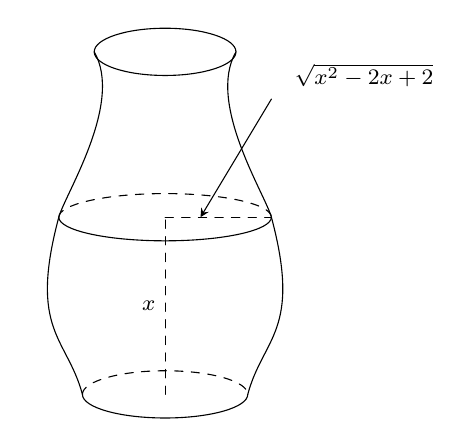
\begin{tikzpicture}[scale=1.5, font=\footnotesize, line join=round, line cap=round, >=stealth]
			\draw (0,1.4) ellipse (0.6cm and 0.2cm);
			\draw[dashed] (-0.9,0) arc (180:0:0.9cm and 0.2cm);
			\draw (-0.9,0) arc (-180:0:0.9cm and 0.2cm);
			\draw[dashed] (-0.7,-1.5) arc (180:0:0.7cm and 0.2cm);
			\draw (-0.7,-1.5) arc (-180:0:0.7cm and 0.2cm);
			\draw (-0.6,1.4).. controls +(-60:0.5) and +(75:0.2)..(-0.9,0)..controls +(-105:1) and +(105:0.5)..(-0.7,-1.5);
			\draw (0.6,1.4).. controls +(-120:0.5) and +(105:0.2)..(0.9,0)..controls +(-75:1) and +(75:0.5)..(0.7,-1.5);
			\draw [dashed](0,0)--(0.9,0) (0,-1.5)--(0,0) node[pos=0.5,left]{$x$};
			\draw [->](0.9,1)--(0.3,0) node[pos=-0.2,right=-0.2]{$\sqrt{x^2-2x+2}$};
	\end{tikzpicture}}
	\shortans{22}
	\loigiai{
		Thể tích của bình hoa là khối tròn xoay sinh bởi $y = \sqrt{x^2-2x+2}$ trên $[0;3]$:
		$$V_{\text{bình}} = \pi \displaystyle\int \limits_{0}^{3} (x^2-2x+2) \mathrm{\,d}x = \pi \left[ \dfrac{x^3}{3} - x^2 + 2x \right]_0^3 = \pi (9 - 9 + 6) = 6\pi.$$
		Mức nước cao bằng $1/3$ chiều cao bình, tức là $h_{\text{nước}} = 1\text{ dm}$. \\
		Thể tích lượng nước trong bình là:
		$$V_{\text{nước}} = \pi\displaystyle \int \limits_{0}^{1} (x^2-2x+2) \mathrm{\,d}x = \pi \left[ \dfrac{x^3}{3} - x^2 + 2x \right]_0^1 = \pi \left( \dfrac{1}{3} - 1 + 2 \right) = \dfrac{4\pi}{3}.$$
		Tỉ lệ phần trăm lượng nước so với thể tích bình hoa là:
		$$\dfrac{V_{\text{nước}}}{V_{\text{bình}}} \times 100\% = \dfrac{\dfrac{4\pi}{3}}{6\pi} \times 100\% = \dfrac{4}{18} \times 100\% = 22,22...\%$$
		Làm tròn đến hàng đơn vị ta được 22.
	}
\end{ex}

\begin{ex}%[2H5C4-5]
	Trong không gian với hệ tọa độ $Oxyz$, cho đường thẳng $d \colon \dfrac{x-1}{1}=\dfrac{y-2}{1}=\dfrac{z}{-2}$. Gọi $(P)$ là mặt phẳng chứa đường thẳng $d$ và tạo với mặt phẳng $(\alpha) \colon x+2y+z-5=0$ một góc có số đo nhỏ nhất. Điểm $M(3;2;1)$ cách mặt phẳng $(P)$ một khoảng bằng bao nhiêu (kết quả làm tròn đến hàng phần trăm)?
	\shortans{1,24}
	\loigiai{
		Đường thẳng $d$ đi qua điểm $A(1; 2; 0)$ và có vectơ chỉ phương $\vec{u}_d = (1; 1; -2)$.\\
		Mặt phẳng $(\alpha)$ có vectơ pháp tuyến $\vec{n}_\alpha = (1; 2; 1)$.\\
		Vì $d \subset (P)$ nên $\vec{n}_P \perp \vec{u}_d$. Góc giữa $(P)$ và $(\alpha)$ nhỏ nhất khi $\vec{n}_P = \big[[\vec{n}_\alpha, \vec{u}_d], \vec{u}_d\big]$.\\
		Ta có:
		\begin{align*}
			[\vec{n}_\alpha, \vec{u}_d] &= (-5; 3; -1).\\
			\vec{n}_P &= \big[[\vec{n}_\alpha, \vec{u}_d], \vec{u}_d\big] = (-5; -11; -8).
		\end{align*}
		Chọn $\vec{n}_P = (5; 11; 8)$.\\
		Mặt phẳng $(P)$ chứa $d$ nên sẽ đi qua điểm $A(1; 2; 0)$. Phương trình tổng quát của $(P)$ là:
		$$ 5(x - 1) + 11(y - 2) + 8(z - 0) = 0 \Leftrightarrow 5x + 11y + 8z - 27 = 0 $$
		Khoảng cách từ điểm $M(3; 2; 1)$ đến mặt phẳng $(P)$ là:
		$$ \mathrm{d}(M, (P)) = \frac{|5 \cdot 3 + 11 \cdot 2 + 8 \cdot 1 - 27|}{\sqrt{5^2 + 11^2 + 8^2}} = \frac{18}{\sqrt{210}} \approx 1{,}2421.$$
	}
\end{ex}

\begin{ex}%[2D1V3-6]
	Doanh nghiệp A độc quyền sản xuất một loại máy tính bảng. Gọi $x$ (nghìn sản phẩm, $0 \le x \le 50, x \in \mathbb{N}$) là số lượng sản phẩm bán ra. Giá bán mỗi sản phẩm phụ thuộc số lượng bán ra theo công thức $p(x)=497-2x$ (nghìn đồng/sản phẩm). Tổng chi phí để sản xuất $x$ nghìn sản phẩm là $C(x)=1000+300x-10x^2+\dfrac{1}{3}x^3$ (triệu đồng). Doanh nghiệp cần sản xuất bao nhiêu nghìn sản phẩm máy tính bảng để thu được lợi nhuận lớn nhất biết chi phí đánh thuế mỗi sản phẩm bán ra là $36$ nghìn đồng.
	\shortans{23}
	\loigiai{
		Doanh thu từ việc bán $x$ nghìn sản phẩm (đổi đơn vị ra triệu đồng): $R(x) = x \cdot p(x) = 497x - 2x^2$. \\
		Thuế cho $x$ nghìn sản phẩm là $T(x) = 36x$ (triệu đồng). \\
		Hàm lợi nhuận $P(x) = R(x) - C(x) - T(x)$:
		\begin{align*}
			P(x) &= (497x - 2x^2) - \left(1000+300x-10x^2+\dfrac{1}{3}x^3\right) - 36x \\
			&= -\dfrac{1}{3}x^3 + 8x^2 + 161x - 1000.
		\end{align*}
		Tính đạo hàm $P'(x) = -x^2 + 16x + 161$. \\
		Giải phương trình $P'(x) = 0 \Leftrightarrow \hoac{&x = 23 \text{ (nhận)} \\ &x = -7 \text{ (loại)}}$. \\
		Ta có các giá trị: $P(0) = -1000$; $P(23) = \dfrac{8638}{3}$; $P(50) = -\dfrac{43850}{3}$.\\
		Bảng biến thiên trên đoạn $[0; 50]$:
		\begin{center}
			
\begin{tikzpicture}
				\tkzTabInit[nocadre=false,lgt=1.5,espcl=3,deltacl=0.9]
				{$x$ /0.6, $P'(x)$ /0.6, $P(x)$ /2.5}   
				{$0$, $23$, $50$}
				\tkzTabLine{,+,$0$,-}
				\tkzTabVar{-/ $-1000$ ,+/ $\dfrac{8638}{3}$ ,-/ $-\dfrac{43850}{3}$}
			\end{tikzpicture}
		\end{center}
		Hàm số đạt giá trị lớn nhất tại $x = 23$. \\
		Vậy doanh nghiệp cần sản xuất $23$ nghìn sản phẩm để lợi nhuận lớn nhất.
	}
\end{ex}

\begin{ex}%[1H8C7-2]
	Cho hình chóp $S.ABCD$ có đáy $ABCD$ là hình vuông cạnh $a$. Cạnh bên $SA$ vuông góc với mặt đáy $(ABCD)$ và $SA=a\sqrt{3}$. Gọi $G$ là trọng tâm của tam giác $SAB$, $A'$ là hình chiếu song song của $G$ lên đường thẳng $SA$ theo phương chiếu $AB$. Trên các cạnh $BC$ và $CD$ lần lượt lấy các điểm $E$ và $F$ sao cho $\widehat{EAF}=45^\circ$. Đặt $BE=x, DF=y$ $(x,y>0)$, gọi $V$ là thể tích của khối chóp $A'.AEF$. Biết $V=\dfrac{a^2(x+y)\sqrt{3}}{m}$, tìm $m$.
	\shortans{18}
	\loigiai{
		\begin{center}
			\begin{tikzpicture}[line join=round, line cap=round,thick,scale=.8]
				\coordinate (A) at (0,0);
				\coordinate (B) at (-2,-3);
				\coordinate (D) at (7,0);
				\coordinate (C) at ($(B)+(D)-(A)$);
				\coordinate (S) at (0,6);
				
				% Xác định các điểm phụ trợ
				\coordinate (M) at ($(A)!0.5!(B)$);
				\coordinate (A') at ($(S)!0.6667!(A)$);
				\coordinate (G) at ($(S)!0.6667!(M)$);
				\coordinate (E) at ($(B)!0.6!(C)$);
				\coordinate (F) at ($(D)!0.43!(C)$);
				
				% Vẽ các nét thấy
				\draw (S)--(B) (S)--(C) (S)--(D) (B)--(C)--(D) (E)--(F);
				% Vẽ các nét khuất
				\draw[dashed,thin] (S)--(A) (A)--(B) (A)--(D) (S)--(M) (A')--(G) (A)--(E) (A)--(F) (A')--(E) (A')--(F);
				
				% Ký hiệu góc vuông
				\pic[draw,thin,angle radius=3mm] {right angle = S--A--D}; 
				\pic[draw,thin,angle radius=3mm] {right angle = S--A--B};
				
				% Vẽ điểm và gán nhãn
				\foreach \i/\g in {S/90,A/135,B/-135,C/-45,D/0,A'/30,G/0,M/135,E/-90,F/0}{
					\draw[fill=black](\i) circle (1.5pt) ($(\i)+(\g:3.5mm)$) node[scale=1]{$\i$};
				}
			\end{tikzpicture}
		\end{center}
		Gọi $M$ là trung điểm $AB$. Trọng tâm $G$ của $\Delta SAB$ nằm trên trung tuyến $SM$ sao cho $\dfrac{SG}{SM} = \dfrac{2}{3}$. \\
		Kẻ $GA' \parallel AB \Rightarrow \dfrac{SA'}{SA} = \dfrac{SG}{SM} = \dfrac{2}{3} \Rightarrow AA' = \dfrac{1}{3}SA = \dfrac{a\sqrt{3}}{3}$. \\
		Diện tích đáy $S_{AEF} = S_{ABCD} - (S_{ABE} + S_{ADF} + S_{CEF}) = a^2 - \dfrac{ax}{2} - \dfrac{ay}{2} - \dfrac{(a-x)(a-y)}{2} = \dfrac{a^2 - xy}{2}$. \\
		Theo bài ra $\widehat{EAF}=45^\circ$. Kẻ góc $\alpha = \widehat{BAE}$, $\beta = \widehat{DAF}$, ta có $\alpha + \beta = 45^\circ$. \\
		$\tan(\alpha + \beta) = 1 \Leftrightarrow \dfrac{\tan \alpha + \tan \beta}{1 - \tan \alpha \tan \beta} = 1 \Leftrightarrow \dfrac{\dfrac{x}{a} + \dfrac{y}{a}}{1 - \dfrac{xy}{a^2}} = 1 \Leftrightarrow a(x+y) = a^2 - xy$. \\
		Do đó diện tích $S_{AEF} = \dfrac{a(x+y)}{2}$. \\
		Thể tích khối chóp $A'.AEF$:
		$$V = \dfrac{1}{3} \cdot AA' \cdot S_{AEF} = \dfrac{1}{3} \cdot \dfrac{a\sqrt{3}}{3} \cdot \dfrac{a(x+y)}{2} = \dfrac{a^2(x+y)\sqrt{3}}{18}.$$
		Suy ra $m = 18$.
	}
\end{ex}

\begin{ex}%[2D6V1-3]
	Một ứng viên tham gia quy trình tuyển dụng gồm ba vòng phỏng vấn liên tiếp. Quy định của quy trình là ứng viên chỉ được đi tiếp vào vòng sau nếu vượt qua vòng trước đó và sẽ bị loại ngay lập tức nếu không đạt ở bất kỳ vòng nào. Giả sử xác suất để ứng viên này vượt qua các vòng như sau:\\
	- Xác suất vượt qua vòng $1$ là $0{,}7$.\\
	- Nếu đã vượt qua vòng $1$, xác suất để vượt qua vòng $2$ là $0{,}6$.\\
	- Nếu đã vượt qua cả vòng $1$ và vòng $2$, xác suất vượt qua vòng $3$ là $0{,}5$.\\
	Biết rằng ứng viên này cuối cùng đã không trúng tuyển (bị loại). Tính xác suất để ứng viên đó bị loại ở vòng $2$ hoặc vòng $3$ (tức là đã vượt qua được ít nhất vòng $1$) (kết quả làm tròn đến hàng phần trăm).
	\shortans{$0{,}62$}
	\loigiai{
		Ta mô tả quá trình phỏng vấn của ứng viên bằng sơ đồ cây như sau (Ký hiệu $V$ là Vượt qua, $F$ là Bị loại):
		\begin{center}
			\begin{tikzpicture}[level 1/.style={sibling distance=5cm},
				level 2/.style={sibling distance=4cm},
				level 3/.style={sibling distance=3cm},
				level distance=2cm,
				thick]
				\node {Bắt đầu}
				child {node {$V_1$}
					child {node {$V_2$}
						child {node {$V_3$ (Đậu)}
							edge from parent node[left] {$0{,}5$}
						}
						child {node {$F_3$ (Loại V3)}
							edge from parent node[right] {$0{,}5$}
						}
						edge from parent node[left] {$0{,}6$}
					}
					child {node {$F_2$ (Loại V2)}
						edge from parent node[right] {$0{,}4$}
					}
					edge from parent node[left] {$0{,}7$}
				}
				child {node {$F_1$ (Loại V1)}
					edge from parent node[right] {$0{,}3$}
				};
			\end{tikzpicture}
		\end{center}
		
		Gọi $L$ là biến cố ứng viên bị loại (không trúng tuyển). Nhìn vào sơ đồ cây, biến cố $L$ bao gồm 3 nhánh kết thúc bằng $F_1$, $F_2$, và $F_3$. Xác suất để ứng viên bị loại là:
		$$\mathrm{P}(L) = 0{,}3 + (0{,}7 \cdot 0{,}4) + (0{,}7 \cdot 0{,}6 \cdot 0{,}5) = 0{,}3 + 0{,}28 + 0{,}21 = 0{,}79.$$
		
		Gọi $T$ là biến cố ứng viên bị loại ở vòng $2$ hoặc vòng $3$ (tức là nhánh đi qua $V_1$ nhưng kết thúc ở $F_2$ hoặc $F_3$). Xác suất của biến cố $T$ là:
		$$\mathrm{P}(T) = (0{,}7 \cdot 0{,}4) + (0{,}7 \cdot 0{,}6 \cdot 0{,}5) = 0{,}28 + 0{,}21 = 0{,}49.$$
		
		Xác suất cần tính là xác suất có điều kiện khi ứng viên đã bị loại:
		$$\mathrm{P}(T|L) = \dfrac{\mathrm{P}(T)}{P(L)} = \dfrac{0{,}49}{0{,}79} = \dfrac{49}{79} \approx 0{,}62.$$
	}
\end{ex}



\Closesolutionfile{ans}

\indapan{6}{ans/ans-62-26-2-HaNoi-KimLien-L3-LC}
\indapan{4}{ans/ans-62-26-2-HaNoi-KimLien-L3-DS}
\indapan{6}{ans/ans-62-26-2-HaNoi-KimLien-L3-KQ}
